\documentclass[11pt,a4paper]{article}
%%%%%%%%%%%%%%%%%%%%%%%%% Credit %%%%%%%%%%%%%%%%%%%%%%%%

% template ini dibuat oleh martin.manullang@if.itera.ac.id untuk dipergunakan oleh seluruh sivitas akademik itera.

%%%%%%%%%%%%%%%%%%%%%%%%% PACKAGE starts HERE %%%%%%%%%%%%%%%%%%%%%%%%
\usepackage{graphicx}
\usepackage{caption}
\usepackage{microtype}
\captionsetup[table]{name=Tabel}
\captionsetup[figure]{name=Gambar}
\usepackage{tabulary}
\usepackage{minted}
\usepackage{amsmath}
\usepackage{fancyhdr}
\usepackage{amssymb}
\usepackage{amsthm}
\usepackage{placeins}
\usepackage{amsfonts}
\usepackage{graphicx}
\usepackage[all]{xy}
\usepackage{tikz}
\usepackage{verbatim}
\usepackage[left=2cm,right=2cm,top=3cm,bottom=2.5cm]{geometry}
\usepackage{hyperref}
\hypersetup{
    colorlinks,
    linkcolor={red!50!black},
    citecolor={blue!50!black},
    urlcolor={blue!80!black}
}
\usepackage{caption}
\usepackage{subcaption}
\usepackage{multirow}
\usepackage{psfrag}
\usepackage[T1]{fontenc}
\usepackage{lmodern}
\usepackage[scaled]{beramono}
% Enable inserting code into the document
\usepackage{listings}
\usepackage{xcolor} 
% custom color & style for listing
\definecolor{codegreen}{rgb}{0,0.6,0}
\definecolor{codegray}{rgb}{0.5,0.5,0.5}
\definecolor{codepurple}{rgb}{0.58,0,0.82}
\definecolor{backcolour}{rgb}{0.95,0.95,0.92}
\definecolor{LightGray}{gray}{0.9}
\lstdefinestyle{mystyle}{
	backgroundcolor=\color{backcolour},   
	commentstyle=\color{green},
	keywordstyle=\color{codegreen},
	numberstyle=\tiny\color{codegray},
	stringstyle=\color{codepurple},
	basicstyle=\ttfamily\footnotesize,
	breakatwhitespace=false,         
	breaklines=true,                 
	captionpos=b,                    
	keepspaces=true,                 
	numbers=left,                    
	numbersep=5pt,                  
	showspaces=false,                
	showstringspaces=false,
	showtabs=false,                  
	tabsize=2
}
\lstset{style=mystyle}
\renewcommand{\lstlistingname}{Kode}
%%%%%%%%%%%%%%%%%%%%%%%%% PACKAGE ends HERE %%%%%%%%%%%%%%%%%%%%%%%%


%%%%%%%%%%%%%%%%%%%%%%%%% Data Diri %%%%%%%%%%%%%%%%%%%%%%%%
\newcommand{\student}{\textbf{Dzaki Gastiadirrijal (122140030)}}
\newcommand{\course}{\textbf{Sistem Teknologi Multimedia (IF25-40305)}}
\newcommand{\assignment}{\textbf{Worksheet 1: Setup Python Environment untuk Multimedia}}

%%%%%%%%%%%%%%%%%%% using theorem style %%%%%%%%%%%%%%%%%%%%
\newtheorem{thm}{Theorem}
\newtheorem{lem}[thm]{Lemma}
\newtheorem{defn}[thm]{Definition}
\newtheorem{exa}[thm]{Example}
\newtheorem{rem}[thm]{Remark}
\newtheorem{coro}[thm]{Corollary}
\newtheorem{quest}{Question}[section]
%%%%%%%%%%%%%%%%%%%%%%%%%%%%%%%%%%%%%%%%
\usepackage{lipsum}%% a garbage package you don't need except to create examples.
\usepackage{fancyhdr}
\pagestyle{fancy}
\lhead{Dzaki Gastiadirrijal (122140030)}
\rhead{ \thepage}
\cfoot{\textbf{Worksheet 1: Setup Python Environment untuk Multimedia}}
\renewcommand{\headrulewidth}{0.4pt}
\renewcommand{\footrulewidth}{0.4pt}

%%%%%%%%%%%%%%  Shortcut for usual set of numbers  %%%%%%%%%%%

\newcommand{\N}{\mathbb{N}}
\newcommand{\Z}{\mathbb{Z}}
\newcommand{\Q}{\mathbb{Q}}
\newcommand{\R}{\mathbb{R}}
\newcommand{\C}{\mathbb{C}}
\setlength\headheight{14pt}

%%%%%%%%%%%%%%%%%%%%%%%%%%%%%%%%%%%%%%%%%%%%%%%%%%%%%%%555
\begin{document}
\thispagestyle{empty}
\begin{center}
	
\includegraphics[scale = 0.15]{Figure/ifitera-header.png}
	\vspace{0.1cm}
\end{center}
\noindent
\rule{17cm}{0.2cm}\\[0.3cm]
Nama: \student \hfill Tugas Ke: \assignment\\[0.1cm]
Mata Kuliah: \course \hfill Tanggal: \today\\
\rule{17cm}{0.05cm}
\vspace{0.1cm}



%%%%%%%%%%%%%%%%%%%%%%%%%%%%%%%%%%%%%%%%%%%%% BODY DOCUMENT %%%%%%%%%%%%%%%%%%%%%%%%%%%%%%%%%%%%%%%%%%%%%
\section{Tujuan Pembelajaran}
Setelah menyelesaikan worksheet ini, mahasiswa diharapkan mampu:
\begin{itemize}
    \item Memahami pentingnya manajemen environment Python untuk pengembangan multimedia
    \item Menginstall dan mengkonfigurasi Python environment menggunakan conda, venv, atau uv
    \item Menginstall library-library Python yang diperlukan untuk multimedia processing
    \item Memverifikasi instalasi dengan mengimpor dan menguji library multimedia
    \item Mendokumentasikan proses konfigurasi dan hasil pengujian dalam format \LaTeX
\end{itemize}

\section{Latar Belakang}
Python telah menjadi bahasa pemrograman yang sangat populer untuk multimedia processing karena memiliki ekosistem library yang sangat kaya. Namun, untuk dapat bekerja dengan multimedia secara efektif, kita perlu mengatur environment Python dengan benar dan menginstall library-library yang tepat.

Manajemen environment Python sangat penting untuk:
\begin{itemize}
    \item Menghindari konflik antar library (dependency conflict)
    \item Memastikan reproducibility dari project
    \item Memudahkan kolaborasi antar developer
    \item Memisahkan project yang berbeda dengan requirement yang berbeda
\end{itemize}

\section{Instruksi Tugas}

\subsection{Persiapan}
\textbf{Sebelum memulai, pastikan Anda telah:}
\begin{itemize}
    \item Menginstall Python 3.8 atau lebih baru di sistem Anda
    \item Memilih salah satu tool manajemen environment: \textbf{conda}, \textbf{venv}, atau \textbf{uv}
    \item Membuka terminal/command prompt
    \item Menyiapkan dokumen \LaTeX\ ini untuk dokumentasi
\end{itemize}

\subsection{Bagian 1: Membuat Environment Python}
Pilih \textbf{SALAH SATU} dari tiga opsi berikut dan ikuti langkah-langkahnya:

\subsubsection{Opsi 1: Menggunakan Conda (Direkomendasikan untuk pemula)}
Jalankan perintah berikut di terminal:

\begin{lstlisting}[language=bash, caption=Membuat environment dengan Conda]
# Membuat environment baru dengan nama 'multimedia'
conda create -n multimedia python=3.11

# Mengaktifkan environment
conda activate multimedia

# Verifikasi environment aktif
conda info --envs
\end{lstlisting}

\subsubsection{Opsi 2: Menggunakan venv (Built-in Python)}
\begin{lstlisting}[language=bash, caption=Membuat environment dengan venv]
# Membuat environment baru
python3 -m venv multimedia-env

# Mengaktifkan environment (Linux/Mac)
source multimedia-env/bin/activate

# Mengaktifkan environment (Windows)
# multimedia-env\Scripts\activate

# Verifikasi environment aktif
which python
\end{lstlisting}

\subsubsection{Opsi 3: Menggunakan uv (Modern dan cepat)}
\begin{lstlisting}[language=bash, caption=Membuat environment dengan uv]
# Install uv terlebih dahulu jika belum ada
# pip install uv

# Membuat environment baru
uv venv multimedia-uv

# Mengaktifkan environment (Linux/Mac)
source multimedia-uv/bin/activate

# Mengaktifkan environment (Windows)
# multimedia-uv\Scripts\activate

# Verifikasi environment aktif
which python
\end{lstlisting}

\textbf{Dokumentasikan di sini:}
\begin{itemize}
    \item Tool manajemen environment yang Anda pilih: \textbf{[uv]}
    \item Screenshot atau copy-paste output dari perintah verifikasi environment
    
\end{itemize}
\begin{figure}[H] 
    \centering
    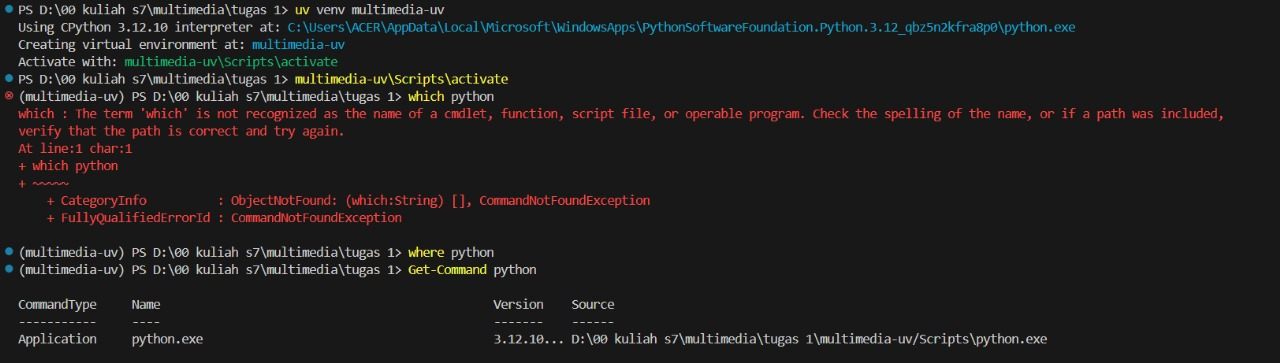
\includegraphics[width=0.8\textwidth]{figure/ss1.jpg}
    \caption{Hasil verifikasi environment dengan uv (which python tidak bisa digunakan di windows)}
    \label{fig:ss1}
\end{figure}

\subsection{Bagian 2: Instalasi Library Multimedia}
Setelah environment aktif, install library-library berikut:

\subsubsection{Library Audio Processing}
\begin{lstlisting}[language=bash, caption=Instalasi library audio]
# Untuk conda:
conda install -c conda-forge librosa soundfile scipy

# Untuk pip (venv/uv):
pip install librosa soundfile scipy
\end{lstlisting}

\subsubsection{Library Image Processing}
\begin{lstlisting}[language=bash, caption=Instalasi library image]
# Untuk conda:
conda install -c conda-forge opencv pillow scikit-image matplotlib

# Untuk pip (venv/uv):
pip install opencv-python pillow scikit-image matplotlib
\end{lstlisting}

\subsubsection{Library Video Processing}
\begin{lstlisting}[language=bash, caption=Instalasi library video]
# Untuk conda:
conda install -c conda-forge ffmpeg
pip install moviepy

# Untuk pip (venv/uv):
pip install moviepy
\end{lstlisting}

\subsubsection{Library General Purpose}
\begin{lstlisting}[language=bash, caption=Instalasi library umum]
# Untuk conda:
conda install numpy pandas jupyter

# Untuk pip (venv/uv):
pip install numpy pandas jupyter
\end{lstlisting}

\textbf{Dokumentasikan di sini:}
\begin{itemize}
    \item Perintah instalasi yang Anda gunakan
    \par 1. Untuk mendownload pip dalam environment multimedia-uv \texttt{.\textbackslash multimedia-uv\textbackslash Scripts\textbackslash python.exe -m ensurepip --upgrade}
    \par 2. pip install librosa soundfile scipy
    \par 3. pip install opencv-python pillow scikit-image matplotlib
    \par 4. pip install moviepy
    \par 5. pip install numpy pandas jupyter

    \item Screenshot proses instalasi atau output sukses
    \begin{figure}[h!]
        \centering
        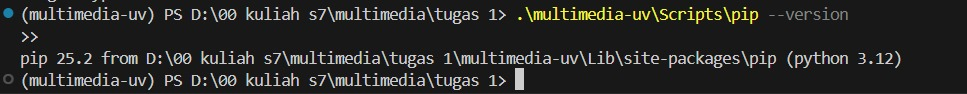
\includegraphics[width=0.8\textwidth]{figure/sspip.jpg}
        \caption{command untuk verifikasi pip dalam env multimedia-uv}
    \end{figure}

    \begin{figure}[h!]
        \centering
        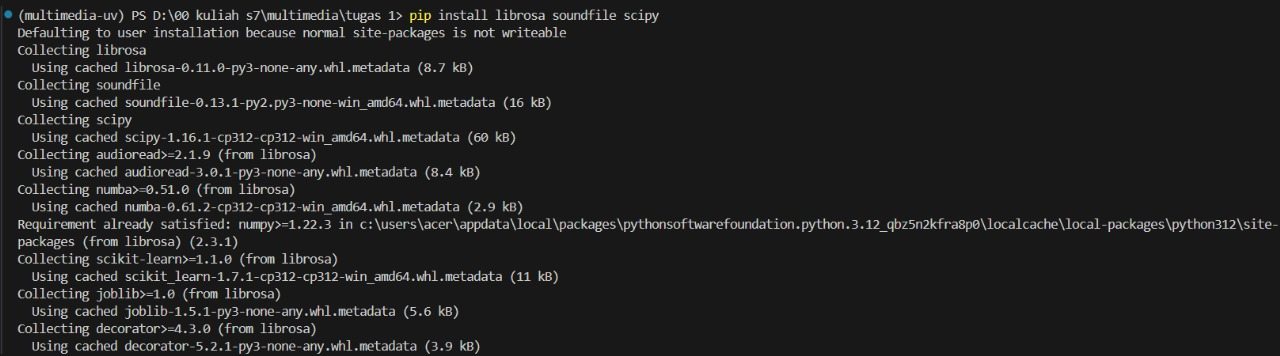
\includegraphics[width=0.8\textwidth]{figure/ss2soundfile.jpg}
        \caption{Proses instalasi librosa soundfile scipy}
    \end{figure}

    \begin{figure}[h!]
        \centering
        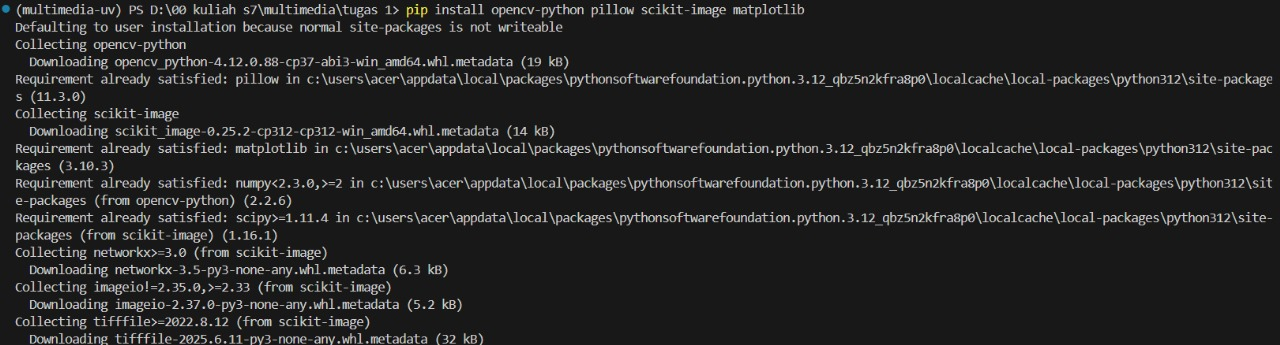
\includegraphics[width=0.8\textwidth]{figure/ss3image.jpg}
        \caption{Proses instalasi opencv-python pillow scikit-image matplotlib}
    \end{figure}

    \begin{figure}[h!]
        \centering
        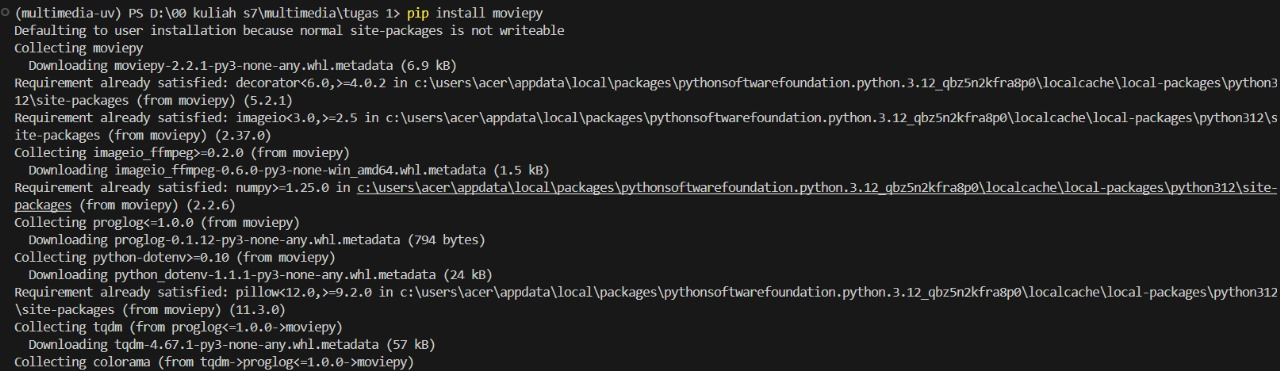
\includegraphics[width=0.5\textwidth]{figure/ss4movie.jpg}
        \caption{Proses instalasi moviepy}
    \end{figure}

    \begin{figure}[H]
        \centering
        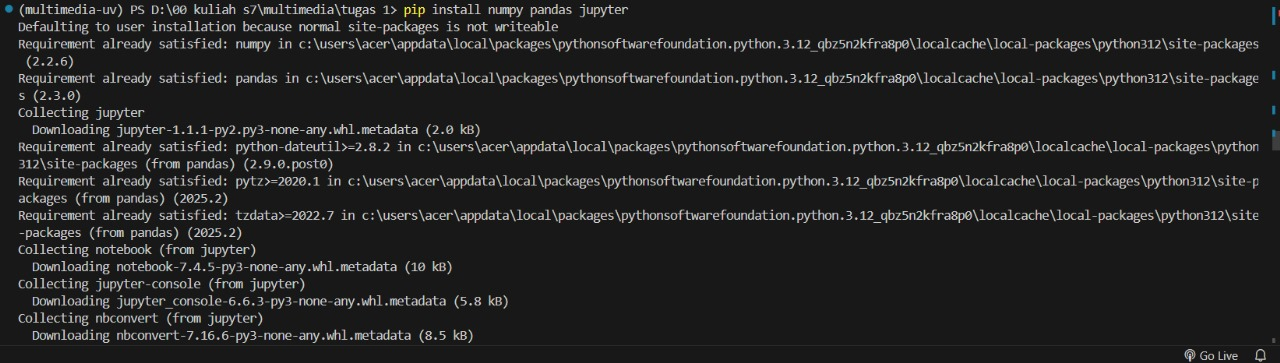
\includegraphics[width=0.6\textwidth]{figure/ss5numpy.jpg}
        \caption{Proses instalasi numpy pandas jupyter}
    \end{figure}

    \item Daftar library yang berhasil diinstall dengan versinya
    \begin{verbatim}
        numpy: 2.2.6
        pandas: 2.3.2
        librosa: 0.11.0
        soundfile: 0.13.1
        scipy: 1.16.1
        opencv-python: 4.12.0
        Pillow: 11.3.0
        scikit-image: 0.25.2
        matplotlib: 3.10.5
        moviepy: 2.1.2
        jupyter-notebook: 7.4.5
    \end{verbatim}
\end{itemize}

\subsection{Bagian 3: Verifikasi Instalasi}
Buat file Python sederhana untuk menguji semua library yang telah diinstall:


\textbf{Jalankan script dan dokumentasikan hasilnya:}
\begin{figure}[H]
    \centering
    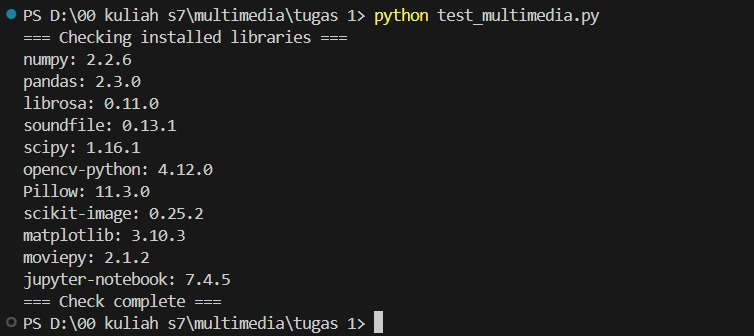
\includegraphics[width=0.6\textwidth]{figure/ss7.jpg}
    \caption{Output script untuk verifikasi instalasi (script dilampirkan pada bagian 4)}
\end{figure}

\subsection{Bagian 4: Simple Test dengan Sample Code}
Buat dan jalankan contoh sederhana untuk setiap kategori multimedia:

\subsubsection{Test Audio Processing}
\begin{lstlisting}[language=Python, caption=Test audio processing sederhana]
import numpy as np
import matplotlib.pyplot as plt

# Generate simple sine wave
duration = 2  # seconds
sample_rate = 44100
frequency = 440  # A4 note

t = np.linspace(0, duration, int(sample_rate * duration))
audio_signal = np.sin(2 * np.pi * frequency * t)

# Plot waveform
plt.figure(figsize=(10, 4))
plt.plot(t[:1000], audio_signal[:1000])  # Plot first 1000 samples
plt.title('Sine Wave (440 Hz)')
plt.xlabel('Time (s)')
plt.ylabel('Amplitude')
plt.grid(True)
plt.savefig('sine_wave_test.png', dpi=150, bbox_inches='tight')
plt.show()

print(f"Generated {duration}s sine wave at {frequency}Hz")
print(f"Sample rate: {sample_rate}Hz")
print(f"Total samples: {len(audio_signal)}")
\end{lstlisting}

\subsubsection{Test Image Processing}
\begin{lstlisting}[language=Python, caption=Test image processing sederhana]
import numpy as np
import matplotlib.pyplot as plt
from PIL import Image

# Create a simple test image
width, height = 400, 300
image = np.zeros((height, width, 3), dtype=np.uint8)

# Add some patterns
image[:, :width//3, 0] = 255  # Red section
image[:, width//3:2*width//3, 1] = 255  # Green section
image[:, 2*width//3:, 2] = 255  # Blue section

# Add a white circle in the center
center_x, center_y = width//2, height//2
radius = 50
Y, X = np.ogrid[:height, :width]
mask = (X - center_x)**2 + (Y - center_y)**2 <= radius**2
image[mask] = [255, 255, 255]

# Display and save
plt.figure(figsize=(8, 6))
plt.imshow(image)
plt.title('Test Image with RGB Stripes and White Circle')
plt.axis('off')
plt.savefig('test_image.png', dpi=150, bbox_inches='tight')
plt.show()

print(f"Created test image: {width}x{height} pixels")
print(f"Image shape: {image.shape}")
print(f"Image dtype: {image.dtype}")
\end{lstlisting}

\textbf{Dokumentasikan hasil eksekusi:}
\begin{itemize}
    \item Screenshot output dari kedua script di atas
    \begin{figure}[H]
        \centering
        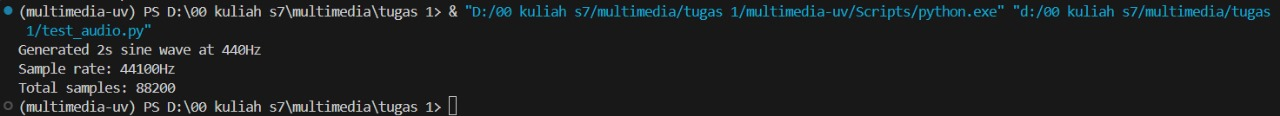
\includegraphics[width=0.8\textwidth]{figure/ss8verif.jpg}
        \caption{Output script Audio}
    \end{figure}
    \begin{figure}[H]
        \centering
        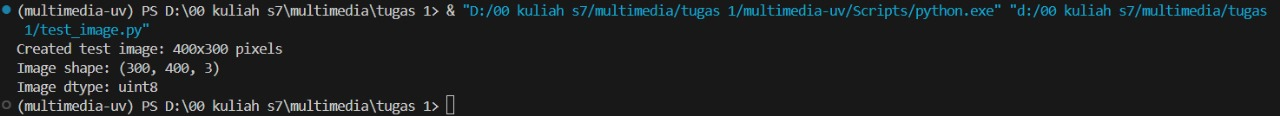
\includegraphics[width=0.8\textwidth]{figure/ss9verif.jpg}
        \caption{Output script Image}
    \end{figure}
    \item Gambar yang dihasilkan (sine\_wave\_test.png dan test\_image.png)
    \begin{figure}[H]
        \centering
        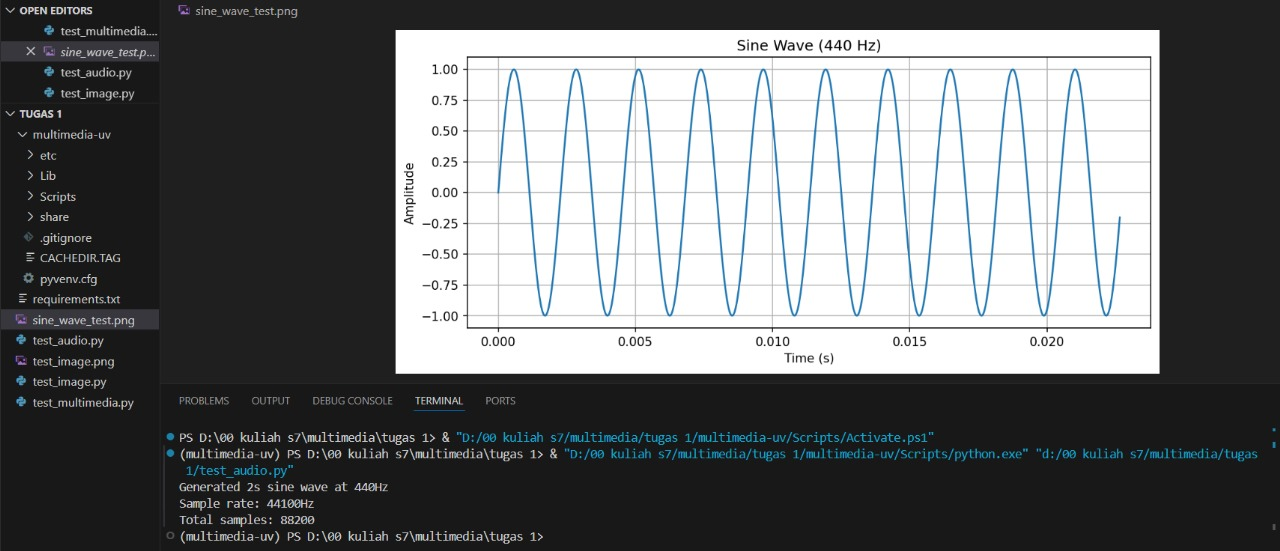
\includegraphics[width=0.8\textwidth]{figure/sine_test.jpg}
        \caption{Output Gambar Audio}
    \end{figure}
    \begin{figure}[H]
        \centering
        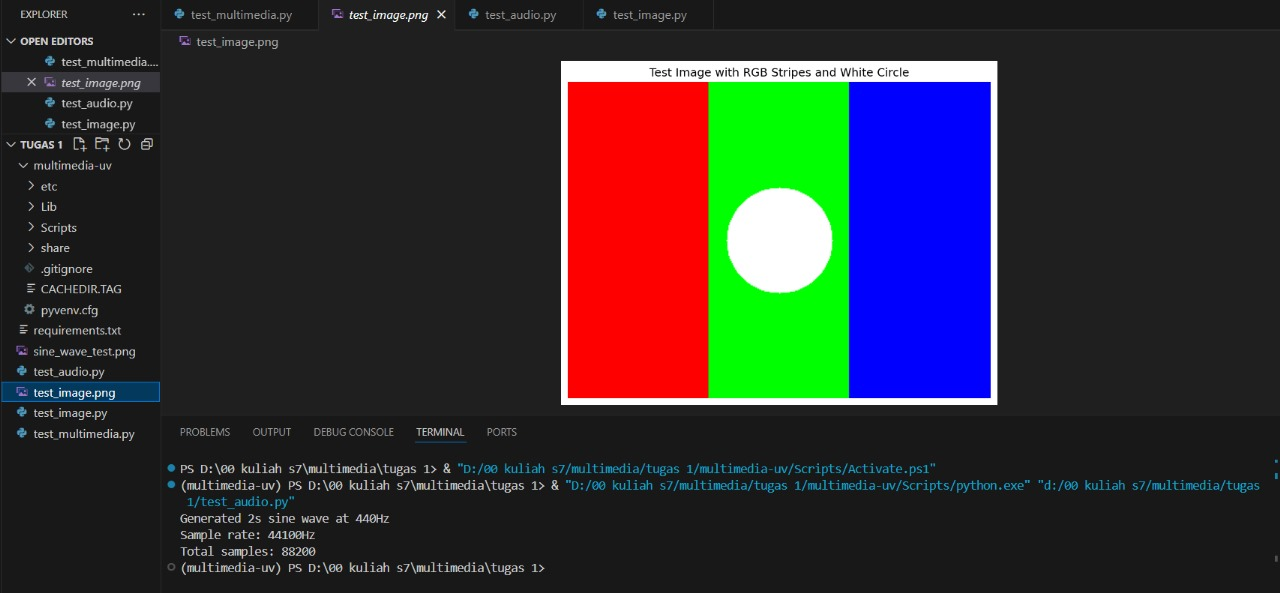
\includegraphics[width=0.8\textwidth]{figure/image_test.jpg}
        \caption{Output Gambar Image}
    \end{figure}
    \item Error message jika ada dan cara mengatasinya
\end{itemize}

\section{Bagian Laporan}

\subsection{Output Verifikasi Instalasi}
\begin{lstlisting}[language=Python, caption=Kode Yang dibuat untuk verifikasi instalasi di test multimedia py]
# check_libs.py
print("=== Checking installed libraries ===")

try:
    import numpy
    print("numpy:", numpy.__version__)
except ImportError:
    print("numpy: NOT INSTALLED")

try:
    import pandas
    print("pandas:", pandas.__version__)
except ImportError:
    print("pandas: NOT INSTALLED")

try:
    import librosa
    print("librosa:", librosa.__version__)
except ImportError:
    print("librosa: NOT INSTALLED")

try:
    import soundfile
    print("soundfile:", soundfile.__version__)
except ImportError:
    print("soundfile: NOT INSTALLED")

try:
    import scipy
    print("scipy:", scipy.__version__)
except ImportError:
    print("scipy: NOT INSTALLED")

try:
    import cv2
    print("opencv-python:", cv2.__version__)
except ImportError:
    print("opencv-python: NOT INSTALLED")

try:
    import PIL
    print("Pillow:", PIL.__version__)
except ImportError:
    print("Pillow: NOT INSTALLED")

try:
    import skimage
    print("scikit-image:", skimage.__version__)
except ImportError:
    print("scikit-image: NOT INSTALLED")

try:
    import matplotlib
    print("matplotlib:", matplotlib.__version__)
except ImportError:
    print("matplotlib: NOT INSTALLED")

try:
    import moviepy
    print("moviepy:", moviepy.__version__)
except ImportError:
    print("moviepy: NOT INSTALLED")

try:
    import notebook
    print("jupyter-notebook:", notebook.__version__)
except ImportError:
    print("jupyter-notebook: NOT INSTALLED")

print("=== Check complete ===")
    
\end{lstlisting}
\textbf{Copy-paste output lengkap dari script \texttt{test\_multimedia.py} di sini:}

\begin{lstlisting}[caption=Output verifikasi instalasi]
[
numpy: 2.2.6
pandas: 2.3.0
librosa: 0.11.0
soundfile: 0.13.1
scipy: 1.16.1
opencv-python: 4.12.0
Pillow: 11.3.0
scikit-image: 0.25.2
matplotlib: 3.10.3
moviepy: 2.1.2
jupyter-notebook: 7.4.5
]
\end{lstlisting}

\subsection{Screenshot Hasil Test}
\textbf{Sisipkan screenshot atau gambar hasil dari:}
\begin{itemize}
    \item Terminal/command prompt yang menunjukkan environment aktif \\
    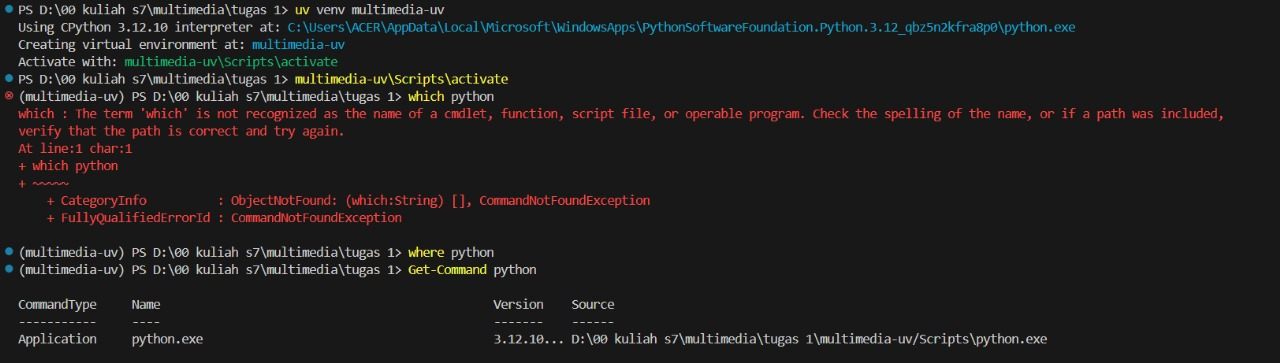
\includegraphics[width=0.8\textwidth]{figure/ss1.jpg}
    \item Output dari script test audio (sine wave plot) \\
    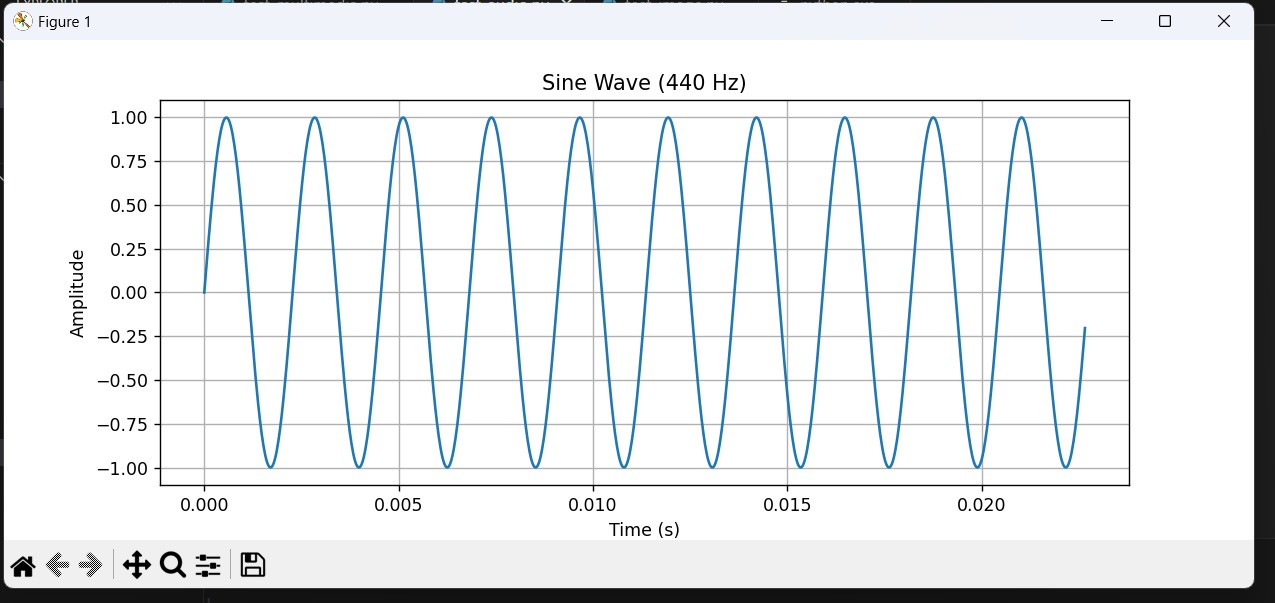
\includegraphics[width=0.5\textwidth]{figure/ss8.jpg}

    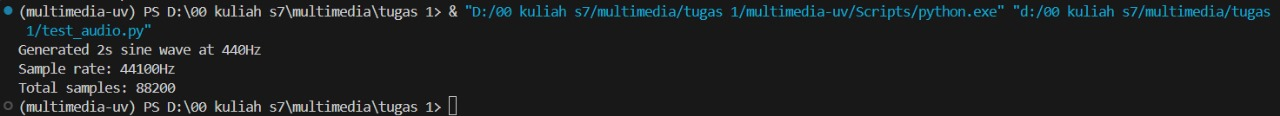
\includegraphics[width=0.8\textwidth]{figure/ss8verif.jpg}
    \item Output dari script test image (RGB stripes dengan circle) \\
    \item 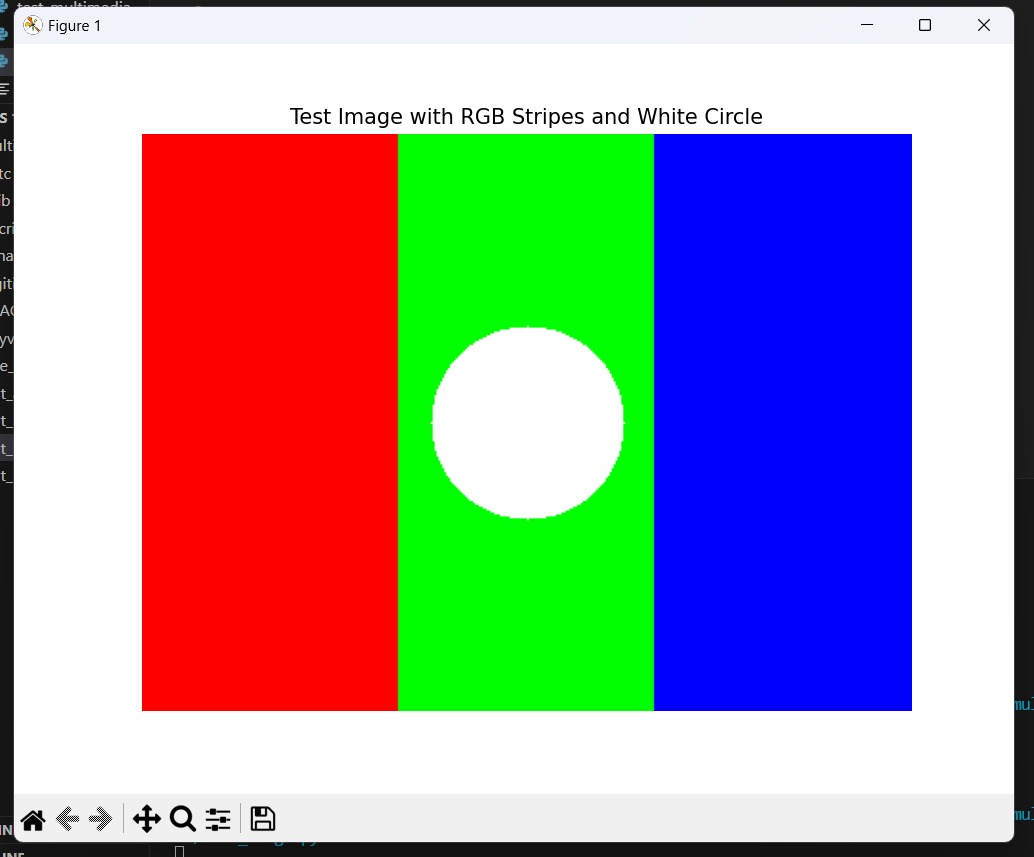
\includegraphics[width=0.5\textwidth]{figure/ss9.jpg}

    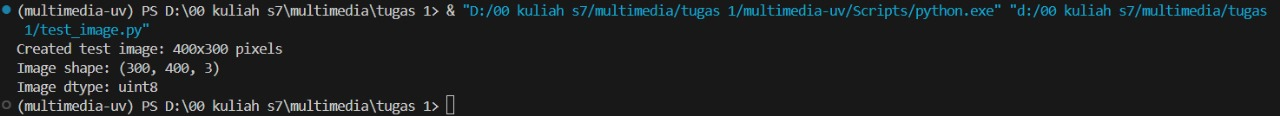
\includegraphics[width=0.8\textwidth]{figure/ss9verif.jpg}
\end{itemize}

\textit{Gunakan perintah \textbackslash\texttt{includegraphics} untuk menyisipkan gambar}

\subsection{Analisis dan Refleksi}
\textbf{Jawab pertanyaan berikut:}

\begin{enumerate}
    \item \textbf{Mengapa penting menggunakan environment terpisah untuk project multimedia?}
    
    \textit{Menurut saya misalnya project saat ini yang saya ingin library x untuk versi 1.x tetapi project lainnya membutuhkan versi 2.x maka otomatis akan tabrakan, dibuatnya environment sendiri untuk mencegah hal seperti itu untuk terjadi agar mereka masing masing punya library sama dengan versi berbeda.}
    
    \item \textbf{Apa perbedaan utama antara conda, venv, dan uv? Mengapa Anda memilih tool yang Anda gunakan?}
    
    \textit{Alasan jujur utama adalah karena tahapan paling mudah diikuti untuk instalasi bagi saya adalah uv lewat bantuan ChatGPT juga. Dan mudahnya uv adalah hanya membuat env kosong -> lalu tinggal instal dengan pip.}
    
    \item \textbf{Library mana yang paling sulit diinstall dan mengapa?}
    
    \textit{Sebenarnya untuk proses instalasi menggunakan pip tidak ada yang rumit hanya berbeda waktu instalasinya. mungkin ini dikarenakan menggunakan uv, masalah yang ditemukan adalah instalasi pada environment yang salah.}
    
    \item \textbf{Bagaimana cara mengatasi masalah dependency conflict jika terjadi?}
    
    \textit{untuk uv, bisa digunakan uv pip check lalu sync requirements.txt untuk disesuaikan. bisa juga menggunakan download versi secara manual atau versi yang diinginkan.}
    
    \item \textbf{Jelaskan fungsi dari masing-masing library yang berhasil Anda install!}
    
    \begin{itemize}
        \item \textbf{librosa}: analisis audio/musik, baca file suara, ekstrak fitur, dan membuat spectrogram.
        \item \textbf{soundfile}: baca/tulis file audio.
        \item \textbf{scipy}: pemrosesan sinyal dan perhitungan ilmiah tambahan.
        \item \textbf{opencv-python}: computer vision, olah citra/video, deteksi objek, deteksi wajah.
        \item \textbf{Pillow}: menambahkan image processing untuk python.
        \item \textbf{scikit-image}: pemrosesan citra ilmiah (segmentasi, transformasi, edge detection).
        \item \textbf{matplotlib}: visualisasi data/gambar dalam bentuk grafik atau plot.
        \item \textbf{moviepy}: edit video sederhana.
        \item \textbf{numpy}: operasi matematika \& array multidimensi.
        \item \textbf{pandas}: olah data tabular.
        \item \textbf{jupyter-notebook}: lingkungan interaktif untuk coding dan visualisasi langsung di browser.
    \end{itemize}
\end{enumerate}

\subsection{Troubleshooting}
\textbf{Dokumentasikan masalah yang Anda hadapi (jika ada) dan cara mengatasinya:}

\begin{itemize}
    \item \textbf{Masalah 1:} \textit{which python tidak bisa digunakan karena tidak ada di versi windows, dan where python tidak ada output} \\
    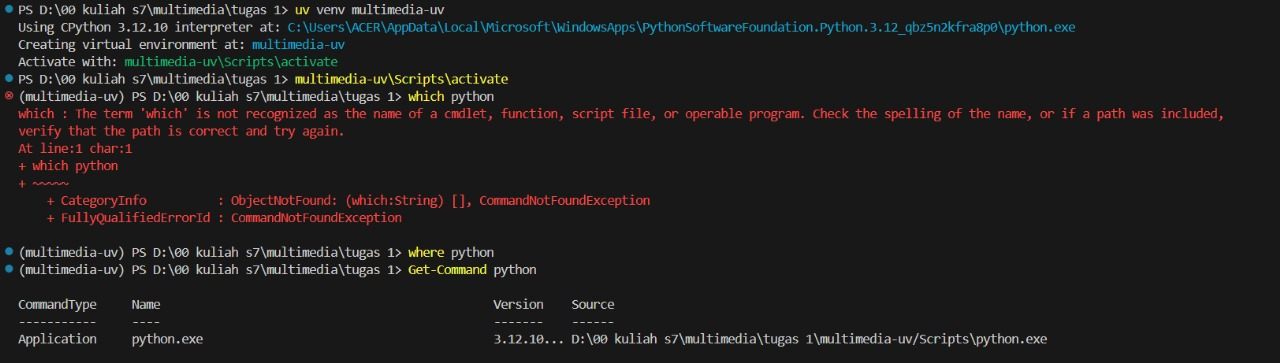
\includegraphics[width=0.9\textwidth]{Figure/ss1.jpg} \\
    \textbf{Solusi:} \textit{Menggunakan where python, lalu menggunakan Command-get python untuk menemukan source python.exe nya}
    
    \item \textbf{Masalah 2:} \textit{Sudah pip instal tetapi tidak terdeteksi di environment multimedia-uv} \\
    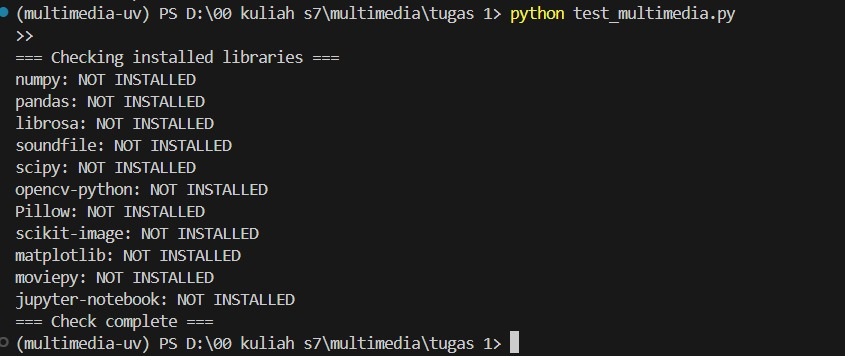
\includegraphics[width=0.9\textwidth]{Figure/masalah2.jpg} \\
    
    \textbf{Solusi:} \textit{Gunakan command 
.\textbackslash multimedia-uv\textbackslash Scripts\textbackslash python.exe -m ensurepip --upgrade 
untuk menginstall pip ke dalam folder environment yang benar.}

\end{itemize}

\section{Export Environment untuk Reproduksi}
Sebagai langkah terakhir, export environment Anda agar dapat direproduksi:

\subsection{Untuk Conda}
\begin{lstlisting}[language=bash, caption=Export conda environment]
conda env export > environment.yml
\end{lstlisting}

\subsection{Untuk venv/uv}
\begin{lstlisting}[language=bash, caption=Export pip requirements]
pip freeze > requirements.txt
\end{lstlisting}

\textbf{Copy-paste isi file environment.yml atau requirements.txt di sini:}

\begin{lstlisting}[caption=Environment/Requirements file]
    anyio==4.10.0
    argon2-cffi==25.1.0
    argon2-cffi-bindings==25.1.0
    arrow==1.3.0
    asttokens==3.0.0
    async-lru==2.0.5
    attrs==25.3.0
    audioread==3.0.1
    babel==2.17.0
    beautifulsoup4==4.13.5
    bleach==6.2.0
    certifi==2025.8.3
    cffi==1.17.1
    charset-normalizer==3.4.3
    colorama==0.4.6
    comm==0.2.3
    contourpy==1.3.3
    cycler==0.12.1
    debugpy==1.8.16
    decorator==5.2.1
    defusedxml==0.7.1
    executing==2.2.0
    fastjsonschema==2.21.2
    fonttools==4.59.1
    fqdn==1.5.1
    h11==0.16.0
    httpcore==1.0.9
    httpx==0.28.1
    idna==3.10
    imageio==2.37.0
    imageio-ffmpeg==0.6.0
    ipykernel==6.30.1
    ipython==9.4.0
    ipython_pygments_lexers==1.1.1
    ipywidgets==8.1.7
    isoduration==20.11.0
    jedi==0.19.2
    Jinja2==3.1.6
    joblib==1.5.1
    json5==0.12.1
    jsonpointer==3.0.0
    jsonschema==4.25.1
    jsonschema-specifications==2025.4.1
    jupyter==1.1.1
    jupyter-console==6.6.3
    jupyter-events==0.12.0
    jupyter-lsp==2.2.6
    jupyter_client==8.6.3
    jupyter_core==5.8.1
    jupyter_server==2.17.0
    jupyter_server_terminals==0.5.3
    jupyterlab==4.4.6
    jupyterlab_pygments==0.3.0
    jupyterlab_server==2.27.3
    jupyterlab_widgets==3.0.15
    kiwisolver==1.4.9
    lark==1.2.2
    lazy_loader==0.4
    librosa==0.11.0
    llvmlite==0.44.0
    MarkupSafe==3.0.2
    matplotlib==3.10.5
    matplotlib-inline==0.1.7
    mistune==3.1.3
    moviepy==2.2.1
    msgpack==1.1.1
    nbclient==0.10.2
    nbconvert==7.16.6
    nbformat==5.10.4
    nest-asyncio==1.6.0
    networkx==3.5
    notebook==7.4.5
    notebook_shim==0.2.4
    numba==0.61.2
    numpy==2.2.6
    opencv-python==4.12.0.88
    packaging==25.0
    pandas==2.3.2
    pandocfilters==1.5.1
    parso==0.8.5
    pillow==11.3.0
    platformdirs==4.3.8
    pooch==1.8.2
    proglog==0.1.12
    prometheus_client==0.22.1
    prompt_toolkit==3.0.51
    psutil==7.0.0
    pure_eval==0.2.3
    pycparser==2.22
    Pygments==2.19.2
    pyparsing==3.2.3
    python-dateutil==2.9.0.post0
    python-dotenv==1.1.1
    python-json-logger==3.3.0
    pytz==2025.2
    pywin32==311
    pywinpty==3.0.0
    PyYAML==6.0.2
    pyzmq==27.0.2
    referencing==0.36.2
    requests==2.32.5
    rfc3339-validator==0.1.4
    rfc3986-validator==0.1.1
    rfc3987-syntax==1.1.0
    rpds-py==0.27.0
    scikit-image==0.25.2
    scikit-learn==1.7.1
    scipy==1.16.1
    Send2Trash==1.8.3
    setuptools==80.9.0
    six==1.17.0
    sniffio==1.3.1
    soundfile==0.13.1
    soupsieve==2.7
    soxr==0.5.0.post1
    stack-data==0.6.3
    terminado==0.18.1
    threadpoolctl==3.6.0
    tifffile==2025.6.11
    tinycss2==1.4.0
    tornado==6.5.2
    tqdm==4.67.1
    traitlets==5.14.3
    types-python-dateutil==2.9.0.20250822
    typing_extensions==4.15.0
    tzdata==2025.2
    uri-template==1.3.0
    urllib3==2.5.0
    wcwidth==0.2.13
    webcolors==24.11.1
    webencodings==0.5.1
    websocket-client==1.8.0
    widgetsnbextension==4.0.14
    
\end{lstlisting}

\section{Kesimpulan}
\textbf{Tuliskan kesimpulan Anda mengenai:}
\begin{itemize}
    \item Pengalaman setup Python environment untuk multimedia \\
    \begin{itshape}
        Proses setup ternyata lebih kompleks dari yang dibayangkan. Meskipun sebagian besar library dapat diinstal dengan mudah menggunakan uv, tetap ada beberapa hal teknis yang perlu diperhatikan supaya environmentnya berjalan stabil.
    \end{itshape}
    \item Persiapan untuk project multimedia selanjutnya \\
    \begin{itshape}
        Untuk persiapan project multimedia berikutnya, saya berencana fokus pada augmented reality (AR). Rencana saya adalah mencari referensi fitur-fitur AR yang pernah dibuat sebelumnya.
    \end{itshape}
    \item Saran untuk mahasiswa lain yang akan melakukan setup serupa \\
    \begin{itshape}
        Jangan ragu menonton tutorial di YouTube atau meminta bantuan dari teman yang sudah bisa melakukannya.
    \end{itshape}
\end{itemize}




\section{Referensi}

Berikut referensi yang digunakan selama proses setup dan troubleshooting Python environment:

\begin{itemize}
    \item \href{https://chatgpt.com/share/68b15fe0-1258-8001-a44f-8431584ab118}{ChatGPT - setup uv dan membuat test multimedia py}
    \item \href{https://chatgpt.com/share/68add498-692c-8001-aba7-ba2e1cd8390c}{ChatGPT - Troubleshooting "which python" yang tidak bisa bekerja}
    \item \href{https://chatgpt.com/share/68add574-3730-8001-990b-85420e938ead}{ChatGPT - Troubleshooting isu instalasi Python/UV environment}
\end{itemize}


\newpage
\bibliographystyle{IEEEtran}
\bibliography{Referensi}
\end{document}